
%----------------------------------------------------------------------------------------
%	Settings and packages
%----------------------------------------------------------------------------------------

\documentclass[10pt]{article}

\usepackage{colortbl}
\usepackage{multirow}
\usepackage[table]{xcolor}
\usepackage{ctable}
\usepackage{wrapfig}
\usepackage[landscape,margin=0.25in,legalpaper]{geometry}

\newcommand{\mcn}[2]{\multicolumn{#1}{l}{#2}}	
\newcommand{\mccn}[2]{\multicolumn{#1}{c}{#2}}
\newcommand{\mcl}[1]{\multicolumn{2}{l}{#1}}
\newcommand{\mclg}[1]{\multicolumn{2}{l}{\gr #1}}
\newcommand{\mcc}[1]{\multicolumn{2}{c}{#1}}
\newcommand{\mccg}[1]{\multicolumn{2}{c}{\gr #1}}
\newcommand{\mr}[1]{\multirow{-2}{*}{#1}}
\definecolor{Gray}{gray}{0.90}
\newcommand{\gr}{\cellcolor{Gray}}

\newcommand{\thickline}{\specialrule{.1em}{.05em}{.05em}}

% column colours
\newcolumntype{g}{>{\columncolor{Gray}}l}
\newcolumntype{w}{>{\columncolor{white}}l}


%\usepackage{geometry}                		% See geometry.pdf to learn the layout options. There are lots.
%\geometry{letterpaper}                    % ... or a4paper or a5paper or ... 
%\geometry{landscape}                		% Activate for for rotated page geometry

%----------------------------------------------------------------------------------------
%	Create new commands
%----------------------------------------------------------------------------------------

% Commands are in LatexCommands.tex. New commands for this file only can be written here.
%\input{/Applications/TeX/Latex_ancillary/LatexCommands.tex}


%----------------------------------------------------------------------------------------
%	Table
%----------------------------------------------------------------------------------------

\begin{document}

\thispagestyle{empty}
{\bf 2008 Deepwell Cup}
\begin{table}[h!]
    \centering
    \begin{tabular}{l g g w w g g w w g g w w}
        \rowcolor{black}\mcn{13}{\color{white}\bf Round 2: Division Finals} \\
        \rowcolor{white}\\
        &  \mccg{Andrew D}&  \mcc{Daniel S}&  \mccg{David D}&  \mcc{Kollin H}&  \mccg{Michael D}&  \mcc{Thomas L} \\\thickline
        {\bf East} &&&&&&&&&&&&\\\hline
          Montreal Canadiens&&&&&&&&&&&&\\
          Philadelphia Flyers & \mr{MTL} & \mr{6} & \mr{MTL} & \mr{6} & \mr{MTL} & \mr{6} & \mr{MTL} & \mr{6} & \mr{MTL} & \mr{6} & \mr{MTL} & \mr{5}\\\hline
          &&&&&&&&&&&& \\\hline
          Pittsburgh Penguins&&&&&&&&&&&&\\
          New York Rangers & \mr{NYR} & \mr{6} & \mr{PIT} & \mr{5} & \mr{NYR} & \mr{7} & \mr{NYR} & \mr{6} & \mr{PIT} & \mr{6} & \mr{PIT} & \mr{6}\\\hline
          &&&&&&&&&&&& \\
        {\bf West} &&&&&&&&&&&&\\\hline
          Detroit Red Wings&&&&&&&&&&&&\\
          Colorado Avalanche & \mr{DET} & \mr{6} & \mr{COL} & \mr{7} & \mr{COL} & \mr{6} & \mr{DET} & \mr{6} & \mr{COL} & \mr{7} & \mr{COL} & \mr{6}\\\hline
          &&&&&&&&&&&& \\\hline
          San Jose Sharks&&&&&&&&&&&&\\
          Dallas Stars & \mr{SJS} & \mr{6} & \mr{SJS} & \mr{6} & \mr{SJS} & \mr{7} & \mr{SJS} & \mr{7} & \mr{DAL} & \mr{6} & \mr{SJS} & \mr{6}\\\hline
          \rowcolor{white}\\
        \rowcolor{black} \mcn{13}{\color{white}\bf Conference Champions} \\
          Eastern & \mclg{MTL} & \mcl{MTL} & \mclg{MTL} & \mcl{MTL} & \mclg{MTL} & \mcl{MTL}\\
          Western & \mclg{DET} & \mcl{SJS} & \mclg{ANA} & \mcl{SJS} & \mclg{SJS} & \mcl{ANA}\\
          Stanley Cup & DET & 6 & MTL & 7 & MTL & 6 & SJS & 7 & SJS & 6 & MTL & 6
    \end{tabular}
\end{table}

\begin{table}[!htb]
\begin{minipage}[t]{.27\linewidth}
{\bf Points}\\
\begin{tabular}{l l}
    Correct team:	& $10$\\
    Correct series length (regardless of series winner):	& $7$\\
    Correct team in a seven game series    & $2$\\
    Stanley Cup champion:	& 25\\
    Stanley Cup runner-up:	& 15\\
\end{tabular}
\hspace{0.5cm}
\begin{wrapfigure}{r}{0.01\textwidth}
    \vspace{-3cm}
	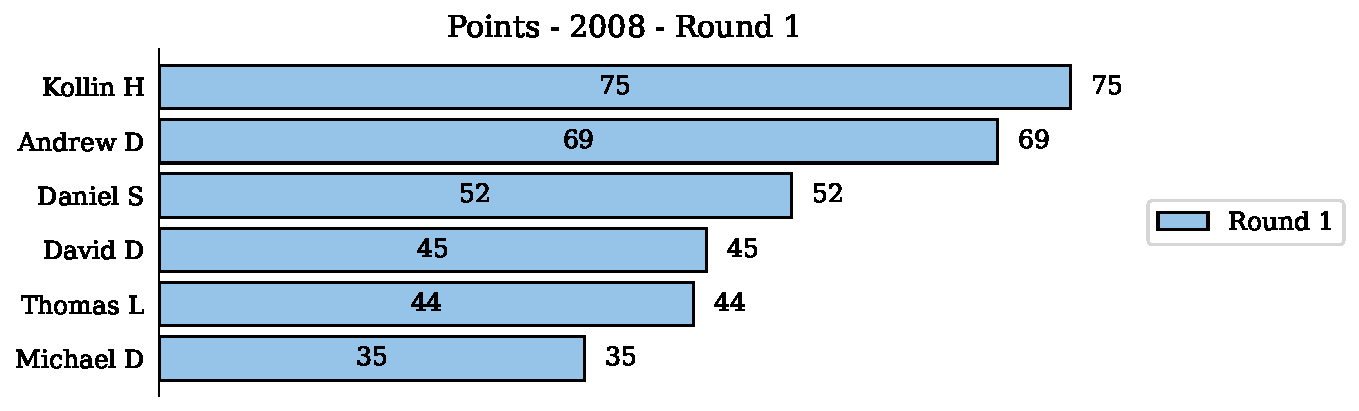
\includegraphics[width=5in]{/Users/daviddeepwell/Documents/Hockey/HockeyPool/DeepwellCup/figures/2008/Points-2008-Round1.pdf}
\end{wrapfigure}
\end{minipage}
\end{table}

\begin{minipage}[t]{.45\linewidth}
{\bf Number of picks per team:}\\
\begin{tabular}{lc | lc | lc | lc }
    MTL & 6 & PIT & 3 & DET & 2 & SJS & 5 \\
    PHI & 0 & NYR & 3 & COL & 4 & DAL & 1 \\
\end{tabular}
\end{minipage}

\end{document}